\documentclass{article}
\usepackage{amsmath}
\usepackage{amssymb}
\usepackage{graphicx}
\usepackage{soul}
\usepackage{anysize} %<-for setting margins
\marginsize {1.6cm}{1.6cm}{2.0cm}{2cm}
\usepackage{color}
\newcommand{\dean}[1]{\textcolor{red}{#1}}
\newcommand{\mike}[1]{\textcolor{green}{#1}}
\newcommand{\parham}[1]{\textcolor{blue}{#1}}
\newcommand{\ken}[1]{\textcolor{cyan}{#1}} 

\title{Responses - Spatiotemporal Multi-Resolution Approximation of the Amari Type Neural Field Model}
\author{ P. Aram, D. Freestone, M. Dewar, K. Scerri, V. Jirsa, D. Grayden, V. Kadirkamanathan}

\begin{document}
    \maketitle

    The authors would very much like to thank the reviewers for their encouraging comments and their efforts to help improve this paper. Please find below the authors responses to the reviewers questions and suggestions regarding the manuscript. 
\\

Best Regards,
\\

Parham Aram.

\section{Handling editor}
\begin{enumerate}
\item Whilst the paper does fit the scope of NI, I agree with R1 and R3, that explicit advantages of going to a multiresolution frame - in addition to the conceptual ones - compared to the prior work based on Gaussian basis functions needs clarification and elucidation.
 
\emph{\parham{The first paragraph of the newly added ``State-space representation'' subsection in the Discussion  highlights the benefits of the MRAIDE compared to the prior work. We also added a paragraph to `` Estimation algorithm'' in the Discussion to clarify the benefits of the novel M-step presented in this work compared to the implementation in Dewar et al.. Please refer to Responses 1 and 5 to R1 for more details.}}


\dean{Parham: Maybe you can make a list of key differences, highlighting the challenges, the technical details, and the benefits that the MRAIDE offers.}

\item  In addition, at least a ``proof of principle" inversion from empirical data would enhance the potential impact of the paper. 


\dean{\emph{The authors agree that the use of empirical data will strengthen the paper. Unfortunately, the authors do not have access to the appropriate data at present. However, we understand that several other groups are now collecting high spatiotemporal resolution data that is appropriate for the methods developed in this paper. We believe that the methods developed in this paper are equally important as the development of high spatiotemporal resolution recording techniques and together, these approaches have enormous potential to answer some of the biggest questions in neuroscience. The ability to use mathematical models as filters, or lenses into the brain if you like, is still a relatively new concept to many members in our community. This new lens allows us to image aspects of neurophysiology of individual subjects that are normally hidden in electrical recordings. Therefore, we believe it is important to continue improve our methods that will lead to the next era in systems neuroscience, where mathematical modelling, experimental measures and model-data fusion will become standard methods. Furthermore, we believe that (good) experimental design is based around the availability of analysis tools. Therefore new imaging tools, like the framework presented in this paper, will lead to new data being collected and potential advances in our collective knowledge of brain function. } }
	
\end{enumerate}

    \section{Reviewer 1}
    
    % It would be useful to mention the above (now below) explicitly in the introduction and try to address them in later sections of the paper.


    \begin{enumerate}
        \item The exposition of the material and the relevant discussion have many similarities with the papers of the same authors (Freestone et al., 2011) and (Dewar et al., 2009) published in Neuroimage and IEEE Trans on Signal Processing  respectively. The authors say the paper at hand is an ``extension'' of Freestone et al. by which I understand they mean the use of a wavelet as opposed to a Gaussian basis for the decomposition. Since the methodology used is the same as in that earlier Neuroimage paper, the paper at hand repeats several of  the results of that previous paper, see sections 3 and 4: equations (2)-(5) and (20) -(33) have already appeared or are very similar to equations in Freestone et al.   
								 
\dean{These first three things are the same point from Reviewer 1.}
	\emph{The earlier papers (Freestone et al., 2011, Dewar et al., 2009) both propose solutions to representing a spatiotemporal field with a finite number of basis functions. Together with this paper, we are building tools that deal with increasing levels of complexity in the spatiotemporal dynamics. The first paper describes key work in the PhD thesis of Dewar, which introduces what we now call a dynamic Galerkin projection. The second in the PhD thesis of Freestone, which recast the estimation problem in the context of neural fields. This paper covers the some of the key results from the PhD thesis of Aram, which details methods for achieving a more accurate representation of the neural fields and an elegant estimation scheme. Each of these steps was a major undertaking and should not be under estimated. There is similarities with the frameworks with all of these papers, where the field is represented by a basis function decomposition. The challenges in forming a multiresolution state-space model included the conceptualisation of the problem, the formulation and derivation of the state-space model, and innovations that make dealing with such a large-scale system feasible. This paper is a result of a concerted effort from our team over a time period of more than two years work. The progress we have made with the earlier papers has made this paper possible, just as we hope that this paper will inspire future work in this direction.}
	        
        \item Section 5 is a review of known results and standard background material from wavelet theory and includes a simple calculation of the Fourier transform of the particular basis used here, which would be more appropriate for an appendix (cf appendix H of the Freestone et al. paper where the Fourier transform of the Gaussian basis functions is calculated).

		% \emph{\parham{Section 5 summarizes important characteristics of B-Spline scaling and wavelet functions which are collected from different references, with an attempt to clarify the inner product and convolution of theses functions (please see R2 comment on ``B-spline calculus''). We think that this brief review can familiarize interested readers  with  B-spline scaling and wavelet functions and direct them to the important literature on this matter. As the reviewer suggested the calculation of the Fourier transform is now moved to the appendix.}}    

\emph{\parham{As the reviewer suggested, moving the calculation of the Fourier transform to the appendix will provide a better flow to the paper. This has been done.}}

\emph{\dean{We understand that this section will not be the central focus of the paper for some members of our research community, however we believe that it is important that this information remains in the paper to allow for implementation without the requirement of digesting information from several texts.}} 

\emph{\dean{We have had similar feedback to your suggestion from our colleagues prior to submission of the paper. Interestingly, the feedback from the people with expertise in wavelet theory thought that the overview of the estimation methods was essential, but the section on wavelets should be reduced. Conversely, people with expertise in the estimation methods thought the overview on wavelets was critical and the section on EM-algorithm should be reduced. We completely appreciate R1 comments and suggestions, but since R2 commented on the usefulness of this section we would very much like to leave it in. We believe that different sections will be valuable for people with different specializations, the synthesis of this information is a valuable contribution for implementation for a wide audience.}}

        \item Section 6 also borrows heavily from Dewar et al, e.g. cf equation (58) of this paper with equation (19) of Dewar et al: the state transition matrix is a perturbation of the corresponding matrix used in that earlier paper. The approach used in both papers seems to be the same with an RTS smoother used in the E-step (this was also used and explained in Freestone et al.) and an M-step optimizing a cost function, quadratic in the parameters, cf. equation (62) with equation (29) of Theorem 2 of Dewar et al. In general, the derivations of section 6 and appendix B follow closely or are very similar to those of Dewar et al.

		\emph{\dean{To clarify the advantage of the M-step over the implementation in Dewar et al. we have added a paragraph to Section 8.1 (now 8.2). Further comments for the reviewer are added below.}}
		
\emph{\dean{The inverse framework in Dewar et al. is based on a general integro-differential equation model, which is not suitable when neural field models are considered. As the result the necessary additions have been made. }}
		
\emph{\dean{This paper has a novel implementation of the M-step, which significantly simplifies the computational complexity of the EM-based algorithm proposed by Dewar et al.. These modifications are significant and crucial for high-dimensional systems. More specifically, implementing the multi-resolution framework introduced in the paper would be impossible without this new contribution. The differences are highlighted in Table.~4 of the manuscript, namely from $O(n_x^4n_{\theta}^2)$ to $O(n_x^2n_{\theta}^2)$, see equation (64) of this paper and equation (31) of Dewar et al, where the static and dynamic components are separated by defining $\boldsymbol \Gamma_1$ and $\mathbf U$ (see equations (65) and (67)). A simplification is also performed to calculate $\boldsymbol\upsilon_0, \boldsymbol\upsilon_1$ (see equations (62) and (63) of this paper and equation (30) of Dewar et al.).} }
		
\emph{\dean{The use of the RTS smoother in the E-step of the EM algorithm for linear state-space models is an effective, standard and widely used approach. In fact, the aim of the IDE representation in a state-space form is to adopt the EM and consequently the RTS smoother in the E-step. The RTS algorithm is presented for completeness to interested readers.} }
		
		\emph{\parham{For linear state-space models, under Gaussian conditions, the lower bound on the log-likelihood function is always quadratic in parameters, and can be solved analytically when the parameters are separable giving results equivalent to the least square estimates. In fact this is one of the advantages of this representation, such a closed form solution for the system's parameters results in significant computational savings.}}
		
        \item Also, Appendix A is the analogue of Appendix D of Freestone et al. and Appendix C includes results known from the literature (as the authors point out).

\emph{\parham{In order to formulate the state-space representation of the multi-resolution neural field model the inner product of the B-spline functions are required. We believe that it is necessary to provide the interested reader with the required tools to implement the algorithm. Appendix D of Freestone et al. and Appendix A herein are only similar in the sense that the inner product of two basis functions are calculated. In Appendix D of Freestone et al. two  n-dimensional Gaussians are considered, while here the inner product of two B-spline functions is calculated. The authors have no objections to remove Appendix C. However as stated above, we think that it would be informative for the broad audience of NeuroImage to include the model specific derivations and some of the well-known formulations of the EM algorithm, since it draws on a wide range of literature.} }

        \item Although I value the use of a wavelet as opposed to a Gaussian basis, the advantages in the context of the analysis of brain imaging data have not been demonstrated and a comparison with the authors' earlier approach has not been performed.  

\emph{\parham{To respond to this important comment we have added ``State-space representation'' subsection into the discussion.}}

				\item{The framework of Freestone et al., seemed not to assume a linear relation between mean membrane potential and firing rate and in that sense the present approach appears more restrictive. }

\emph{\dean{The linear activation function in the estimation algorithm was made out of necessity. This was due to the high dimensionality and associated computational demands of the estimation problem.}}

\emph{\dean{The authors would like to point out that the derivation of the state-space multi-resolution model was made general for all possible activation functions. This derivation is perhaps the most important contribution of the paper \parham{not sure about this because we have already done the derivation in Freestone 2011}. We understand that all physical systems are nonlinear. However, we also understand that linear approximations are often required in engineering for useful models. In the introduction to the estimation section, we have attempted to discuss this issue with regard to forward vs. inverse modelling. \parham{We believe that the linear model is more acceptable for inverse modelling, but understand it is required for forward modelling. ??} For example, in a forward model the nonlinearity is required to prevent negative firing rates. However in the inverse case, the physiology naturally restricts firing rates to be positive. Furthermore, in the mean field case, we do not expect firing rates of all neurons to be zero or all neurons to be simultaneously firing at their maximal rate. Therefore, a linear model may suffice to image a multi-resolution neural field and physiological parameters using electrophysiological data .}}
				
\emph{\dean{Given restrictions of computational complexity, the choice of whether to use the framework presented in Freestone et al. or the current paper may boil down to a trade-off between temporal accuracy and spatial accuracy. Furthermore, the proven convergence of estimation algorithms for linear systems may actually lead to more accurate models given a closed-loop scheme. This is due to the correction step in the algorithm where model error is reduced using measurements.\parham{not sure this is due to the correction step, the correction step of this paper and Freestone 2011 are the same due to the linearity of the observation equation.}}}
				

        \item The authors say that a multi-resolution approach would explain the``organizational level of the brain at which cognition and behaviour are best explained'' but it is unclear what the alternative levels considered here are and what the significance of the results obtained is.

\dean{\emph{Within our framework the alternate levels are defined by the spatial scales of the wavelet decomposition. The significant result is the formulation of a model when various spatial scales of a neural field can be simultaneously represented. The ability to image the multi-dimensional neural field will lead to a better understanding of the important spatial scales when neural information processing occurs.  }}

				\item Similar claims to the ones mentioned here regarding  implications for ``patient-specific'' modelling have also been made in Freestone et al., so it is not clear how these relate to the current multi-resolution approach and also such remarks might look too ambitious given that only synthetic data with fixed parameters are considered.
				
				\dean{\emph{Please refer to Response 2 to the handling editor.}}
				
				\item The comments about model complexity and parsimony on p.13 are somehow vague as these quantities are undefined.
				
				% \emph{\parham{some notes to be added to the manuscript: Parsimony: as few as necessary variables to describe a phenomenon, complexity: to add detail description to the model to increase its accuracy with the natural phenomenon, finding a balance between complexity and parsimony is crucial. By parsimony we sacrifice realism ...  }}
				
				\emph{\ken{To clarify this comment, a short paragraph has been included in section 6 to better explain the modeling choice facing every user, that is; choosing between a more parsimonious or more complex model structure.  For the audience with less experience in system identification, a reference with further information regarding this topic has also been included.}}
				
				\item Also, the comments on large scale networks and delays made on p.20 look irrelevant to the present framework.
				
				\emph{\parham{We have omitted the last paragraph of the discussion on delays in large scale networks.}}
				
				\item Much of the discussion of the last section focuses on technical issues, while the discussion of the observation kernel chosen on p.17 is limited.
				
				\emph{\parham{We have added a paragraph in new subsection ``State-space representation'' in the Discussion, regarding the choice of the observation kernel.}}

    \end{enumerate}
    
    \section{Reviewer 2}
    
\begin{enumerate}
    \item As a minor comment, I would suggest changing the notation for the scaling and wavelet coefficients in Eq. (6), for example into normal lowercase `a' and `c', respectively. The $\beta$ might be confused by B-spline notation. 

	\emph{\parham{We have changed the scaling and wavelet coefficients into normal lowercase `a' and `c', respectively.}}

\item For the discussion, it might be useful to add a sentence that the basis structure (i.e., non-redundant, versus a (tight) frame representation) is a requirement for this framework.

\emph{\parham{We have added a sentence to Sect 8.1 (now 8.2) for the basis structure requirement.}}



\item A small comment might also be considered for Sect 8.2: it is possible to apply other than dyadic subsampling schemes in multiple dimensions, which leads to less wavelet subbands. For example, in 2D, the quincunx scheme is well-known to have better isotropic properties. Unfortunately, in 3D, it is not possible to have a subsampling operator (acting on a Cartesian sampling lattice) that is performing subsampling at equal rate in each dimension at each iteration, see Van De Ville et al,`On the multidimensional extension of the quincunx subsampling lattice', IEEE SPL, 12:2, pp.  112-115, 2005, for a comment on this. 

\emph{\parham{We have added this comment to Sect 8.2 (now 8.3).}}


 % 
 % \begin{figure*}[!ht]
 % \begin{center}
 % 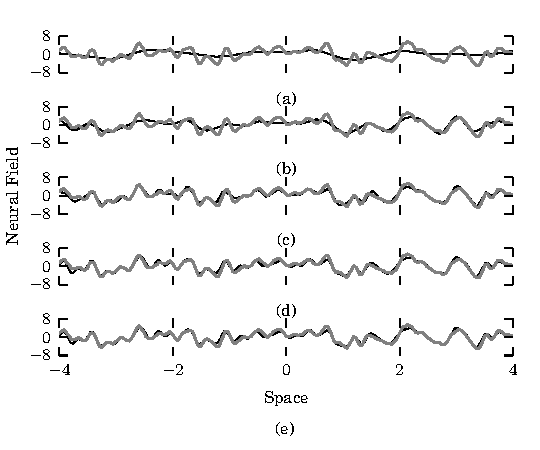
\includegraphics{./Graph/pdf/fig1.pdf} 
 % \end{center}
 % \caption{}
 % \label{fig:Figure1}
 % \end{figure*}

 

\end{enumerate}  

    \section{Reviewer 3}  
    \subsection{Main Concerns}
		\begin{enumerate} 
			\item I am not at all sure that isotopic scaling of the multiresolution is appropriate for brain connections, but I cannot say at this point that it is not.
			
			\emph{\parham{It is generally accepted that the intracortical connectivity structure is isotropic, however, as the reviewer pointed out this is not the case  for corto-cortical connectivity. The presented framework is also valid for other connectivity kernels provided they are spatially homogeneous and that they can be approximated by a set of weighted isotropic basis functions. The connectivity kernel can take any arbitrary shapes but this may require more basis functions to accurately estimate the kernel.}}
			 
			\item This model cries out for validation in real neuronal systems, but alas, at this point we only see convergence to synthetic data.   
			  
			 \emph{\parham{Please refer to Response 2 to the handling editor. Further comments are also added below.}}
			
			 \emph{\parham{The authors appreciate that the only way to truly validate the proposed framework is with real data. However, before validating the method on real data we believe that it is essential to first validate the estimation method using accepted models and synthetic data, where the true and estimated parameters can be compared. The title of the manuscript was chosen such that to reflect this fact, stating this is a multi-resolution framework for Amari type neural field model. In an effort to make the method employed in the paper more explicit, we have added ``data was generated synthetically using Amari neural field model'' to the Result section.}}  
			
			\item This audience needs to have all symbols, including commonly used ones such as `equality over distribution', double font domains like R and Z, and jargon terms such as `lead field'.
			
			\emph{\parham{ We have defined independent and identically distributed (i.i.d.) random variables under Eq. (5). The double font domains are added to Table.1. A brief description of `lead field' is also added below Eq. (5).}}  
			
			\item Frankly, I would off-load all of the very difficult mathematics to the appendices and supplementary data, and focus a NeuroImage paper on the results of image analysis. 
			
			\emph{Response here.}
			
			\item Contrasting, for example, this multiresolution method with Freestone's 2011 results would be helpful for continuity.
			
			\emph{Response here.}
			
			\item I would also recommend archiving code that, for instance generates figure 11, so that the readership has a chance to replicate these findings, and adapt this method to their own data.
			
 			\emph{\parham{We have added a footnote on page 17 : The Python source code for our numerical simulations is available from the authors on request.}}
 		
			                                       
			\end{enumerate}  
			\subsection{Moderate Concerns} 
			\begin{enumerate} 
			 \item Page 2: the authors should clearly define the difference between neural field and neural mass models.
			
			\emph{\parham{We have added the following paragraph on page 2: The main difference between these two classes is that neural field models describe the spatiotemporal evolution of a particular variable such as firing rate, membrane voltage or synaptic activity defined as the statistical expectation taken over a neural population while neural mass models describe such a quantity over time only, assuming that neurons are localized at approximately the same spatial location.}}
			
			\item Eqn 3: theta needs indexing 
 
			\emph{\parham{Authors think that the reviewer is after Eqn 2. for the correction.  We have rewritten Eqn 2 by removing the parameter $\theta$ in order to be consistent with the rest of equations in the manuscript and we have described the coupling strength or synaptic efficiency within the text under Eq 2.}}
 			
			\item Define first and second order synaptic responses (used in figure 2 to explain text that does not refer to these terms)
			
			\emph{\parham{Definitions of first and second order synaptic responses have been added to the text under Eq 2.}}
			
			\item{Eqn 9: the state variables $x$ seem to arise without distinction from $v$}  
			
			\emph{The units of $x$ are also Volts. However the states are weights for particular levels of resolution, where $v$ is the total net field. We have added a sentence to add clarification. \parham{please dont forget to add this to manuscript}}
			
			\item Between eqn 19 and 20 change
			`write the neural field and connectivity kernel decomposition' To `write the connectivity kernel and neural field decomposition'
			To maintain order with eqns 20 and 21.

			\emph{\parham{We have changed the text to `the connectivity kernel and neural field decomposition' to maintain order with eqns 20 and 21.}}
			
			 
			 \end{enumerate}  
			\subsection{Trivia}
			\begin{enumerate}
			 \item 	Define `one-off' on pg 16 

 			\emph{Response here.}

  		\item Figure 8 is referred to in the text out of order

  			\emph{\parham{The cross-referencing has been corrected.}}
			 
			\item Pg 19: `stationary point i.e. global' should be `stationary point, i.e. a global'

			\emph{\parham{We have changed the text to `stationary point, i.e. a global'.}}			
			                   
			
			 
				\end{enumerate} 
				
			
\end{document}